\documentclass[final]{article}

\usepackage{APS360}
\usepackage[utf8]{inputenc}
\usepackage[T1]{fontenc}
\usepackage{hyperref}
\usepackage{url}
\usepackage{booktabs}
\usepackage{amsfonts}
\usepackage{nicefrac}
\usepackage{microtype}
\usepackage{xcolor}
\usepackage{graphicx}
\usepackage{tikz}
\usetikzlibrary{positioning, arrows.meta, fit, backgrounds}
\renewcommand{\arraystretch}{0.88}
\setlength{\abovecaptionskip}{3pt}
\setlength{\belowcaptionskip}{0pt}

\title{Mini-VLM: Progress Report}

\author{%
  Oliver Petrovic \\
  1008923042, oliver.petrovic@mail.utoronto.ca\\
  \url{https://github.com/Olipet24/mini-vlm}\\
}

\begin{document}

\maketitle

\vspace{-0.5in}

\section*{Introduction}

Modern Vision-Language Models (VLMs) are massive, requiring billions of parameters and huge GPU
resources that make them impossible to run on everyday hardware, as well as extremely long to train. Mini-VLM is a compact
VLM for Visual Question Answering (VQA) constrained to a strict \textbf{100MB storage budget}, where given a $224\times224$ image and a free-form text question, the model
outputs one of the 1000 most common VQA answers. Running AI models on
resource-constrained hardware requires aggressive compression, and mapping raw pixels with free-form text jointly requires learned, non-linear visual and linguistic representations that hand-crafted approaches cannot approximate \cite{goyal2017making}. Rather than shrinking a Transformer post hoc, our core contribution is an \emph{RWKV pipeline}. RWKV is a novel architecture that combines the parallelizable training of Transformers with the efficient linear-time inference of Recurrent Neural Networks \cite{peng2023rwkv}. Using an RWKV spatial bridge and language core gives linear-time cost in sequence length, replacing the standard quadratic MLP-to-Transformer approach used by models like LLaVA \cite{liu2023visual}.

\section*{Data Processing}

We use the official \textbf{VQA v2.0} dataset (questions/annotations over COCO images), processed
in two steps: (1) collapse free-form answers to a \textbf{top-1000
most-common-answer classification} problem, built from the frequency distribution over the full
443{,}757-example train2014 pool (87.47\% coverage), dropping examples outside that vocabulary;
(2) resize/normalize images to $224\times224$ and pass them through the frozen vision encoder
\emph{once, offline}, caching the resulting $576\times7\times7$ FP16 feature map so training
never re-runs the encoder.

\begin{table}[!htbp]
\centering
\footnotesize
\begin{tabular}{lr}
\toprule
Statistic & Value \\
\midrule
Train / val / test size & 368{,}751 / 19{,}407 / 186{,}489 \\
Unique images (train+val; test) & 82{,}575; 40{,}404 \\
Cached FP16 feature tensors & 122{,}979 \\
Answer-type mix (yes/no : other : number) & 43.1\% : 43.5\% : 13.4\% \\
Question length (words), mean [min, max] & 6.1 [2, 22] \\
Top-1000 answer coverage (train2014 pool) & 87.47\% \\
\bottomrule
\end{tabular}
\caption{Full-scale dataset statistics (\texttt{outputs/processed\_full/dataset\_stats.json}).}
\label{tab:stats}
\end{table}

\textbf{Train/val/test split.} \texttt{train}/\texttt{val} are disjoint samples from the
official \emph{train2014} pool while \texttt{test} is sampled entirely from \emph{val2014}, making the images
and questions never seen during training or hyperparameter selection, our stand-in for
``never-before-seen'' data. In addition, we plan to create an additional smaller test dataset consisting of around 100 custom images, questions and answers for final model performance testing.

\begin{figure}[!htbp]
  \centering
  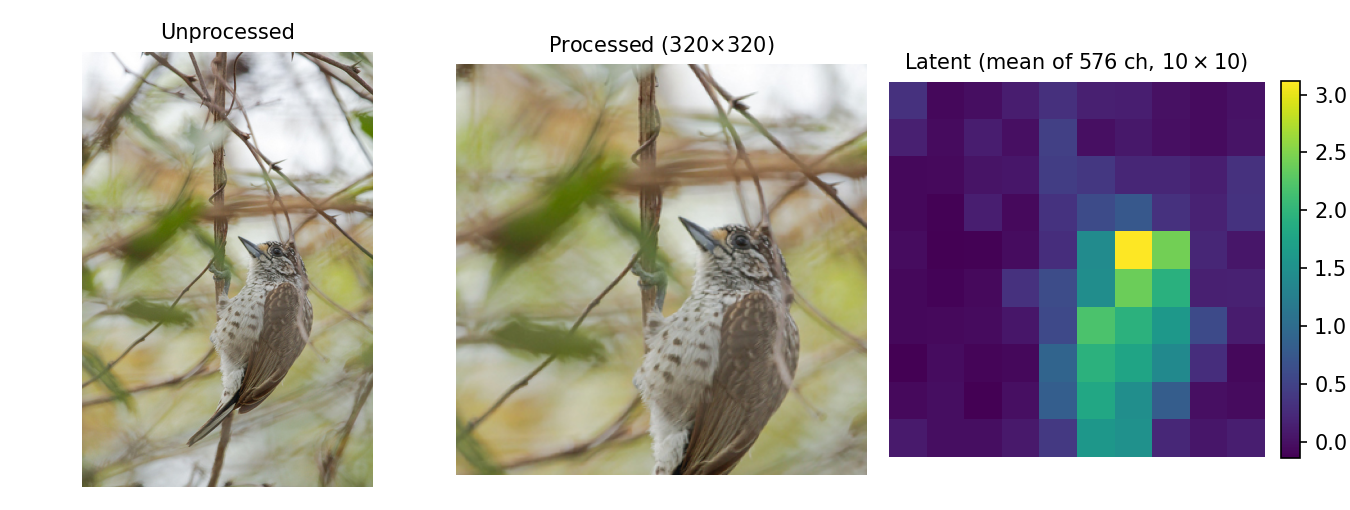
\includegraphics[height=3.5cm]{figures/bird_vision_latents.png}
  \caption{Unprocessed, processed, and encoded latent image, with the following question ``What color is this bird?'' and associated answer
  (class \texttt{white and brown}, one of the top-1000 answer classes).}
  \label{fig:sample}
\end{figure}

\textbf{Challenges.} Downloading/extracting the full $\sim$123,000-image COCO zip archives once was not error-free: a batch of cached
feature tensors was silently corrupted, spiking training loss until we added a feature-integrity
check that now runs before training.

\section*{Baseline Model}
\begin{figure}[!htbp]
  \centering
  \resizebox{\linewidth}{!}{%
  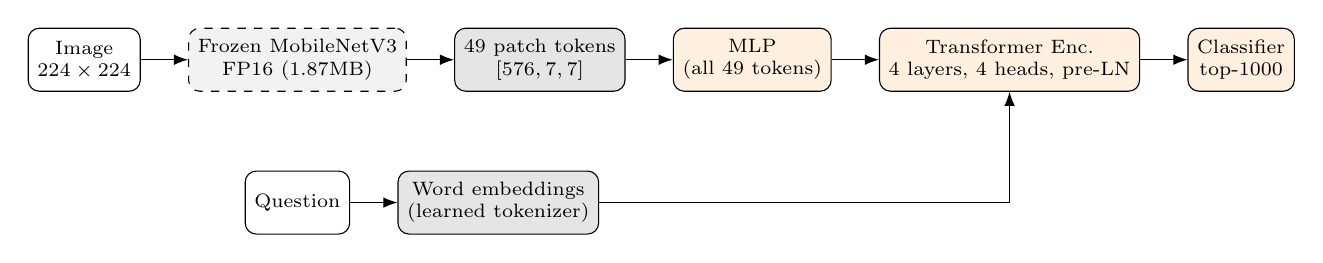
\begin{tikzpicture}[
      node distance=5mm and 6mm,
      box/.style={draw, rounded corners, align=center, minimum height=0.8cm, font=\scriptsize},
      frozen/.style={box, dashed, fill=gray!10},
      base/.style={box, fill=orange!12},
      shared/.style={box, fill=gray!20},
      arr/.style={-{Latex[length=1.8mm]}}
    ]
    % Nodes
    \node[box] (img) {Image\\$224\times224$};
    \node[frozen, right=of img] (enc) {Frozen MobileNetV3\\FP16 (1.87MB)};
    \node[shared, right=of enc] (tok) {49 patch tokens\\$[576,7,7]$};
    
    \node[box, below=1cm of enc] (q) {Question};
    \node[shared, right=of q] (qtok) {Word embeddings\\(learned tokenizer)};

    \node[base, right=of tok] (proj) {MLP\\(all 49 tokens)};
    \node[base, right=of proj] (xfmr) {Transformer Enc.\\4 layers, 4 heads, pre-LN};
    \node[base, right=of xfmr] (ans) {Classifier\\top-1000};

    % Edges
    \draw[arr] (img) -- (enc);
    \draw[arr] (enc) -- (tok);
    \draw[arr] (q) -- (qtok);
    \draw[arr] (tok) -- (proj);
    \draw[arr] (proj) -- (xfmr);
    \draw[arr] (xfmr) -- (ans);
    \draw[arr] (qtok) -| (xfmr.south);
  \end{tikzpicture}%
  }
  \caption{Baseline Model pipeline. Keeping the same frozen encoder, the RWKV bridge/core is replaced with an MLP and a standard multi-head-attention Transformer to isolate the design's contribution.}
  \label{fig:pipeline_baseline}
\end{figure}
The baseline is the ``naive integration'' control group from the proposal: the same frozen
vision encoder, but a plain \textbf{MLP} maps all 49 spatial patch tokens into a standard \texttt{nn.TransformerEncoder} (4 layers, 4 heads,
$d_{model}=128$, pre-LN, Figure~\ref{fig:pipeline_baseline}) alongside the question's word embeddings which is then classified into 1000 answers, requiring no tuning beyond standard
defaults (AdamW, $lr=3\times10^{-3}$).

\textbf{Quantitative results.} Trained for 10 epochs ($587.9$s $\approx$9.8 min) on the full
training pool, the baseline reaches \textbf{47.38\%} held-out test accuracy (2{,}574{,}696
params, 9.84MB) against a \textbf{21.84\%} majority-class floor (Table~\ref{tab:comparison}).
From the graphs, the validation loss is still falling at epoch 10 (1.89$\to$1.55), but the sloper is flattening, indicating it is not yet overfitting.

\textbf{Qualitative results.} Table~\ref{tab:qualitative} (``baseline'' column) shows
representative predictions, and is further discussed in the \textbf{Qualitative results} section of the Primary Model.

\section*{Primary Model}
\label{sec:primarymodel}
\begin{figure}[!htbp]
  \centering
  \resizebox{\linewidth}{!}{%
  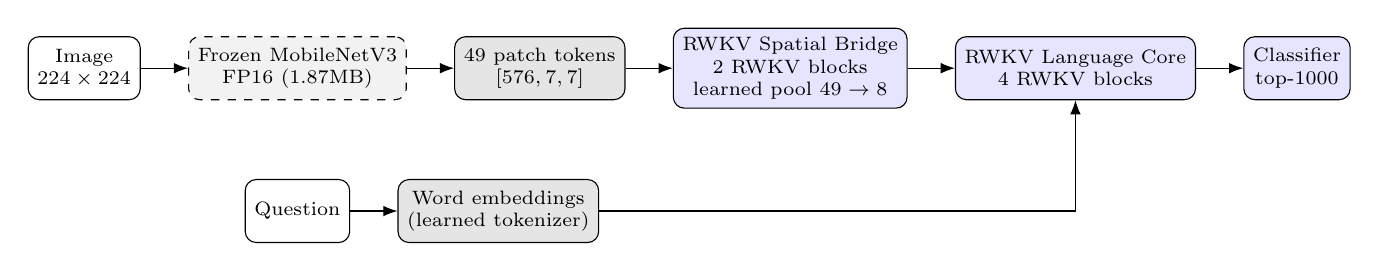
\begin{tikzpicture}[
      node distance=5mm and 6mm,
      box/.style={draw, rounded corners, align=center, minimum height=0.8cm, font=\scriptsize},
      frozen/.style={box, dashed, fill=gray!10},
      primary/.style={box, fill=blue!10},
      shared/.style={box, fill=gray!20},
      arr/.style={-{Latex[length=1.8mm]}}
    ]
    % Nodes
    \node[box] (img) {Image\\$224\times224$};
    \node[frozen, right=of img] (enc) {Frozen MobileNetV3\\FP16 (1.87MB)};
    \node[shared, right=of enc] (tok) {49 patch tokens\\$[576,7,7]$};
    
    \node[box, below=1cm of enc] (q) {Question};
    \node[shared, right=of q] (qtok) {Word embeddings\\(learned tokenizer)};

    \node[primary, right=of tok] (bridge) {RWKV Spatial Bridge\\2 RWKV blocks\\learned pool $49\to8$};
    \node[primary, right=of bridge] (core) {RWKV Language Core\\4 RWKV blocks};
    \node[primary, right=of core] (ans) {Classifier\\top-1000};

    % Edges
    \draw[arr] (img) -- (enc);
    \draw[arr] (enc) -- (tok);
    \draw[arr] (q) -- (qtok);
    \draw[arr] (tok) -- (bridge);
    \draw[arr] (bridge) -- (core);
    \draw[arr] (core) -- (ans);
    \draw[arr] (qtok) -| (core.south);
  \end{tikzpicture}%
  }
  \caption{Primary Model pipeline. The frozen vision encoder runs once offline, and the model compresses 49 spatial tokens to 8 language-aligned tokens before feeding them into the linear-time RWKV stack.}
  \label{fig:pipeline_primary}
\end{figure}

\begin{table}[!htbp]
\centering
\footnotesize
\resizebox{\linewidth}{!}{%
\begin{tabular}{lrrrrrrr}
\toprule
Model & Params & Size & Test acc. & Test loss & Acc.\ y/n & Acc.\ other & Acc.\ num.\\
\midrule
Majority-class floor & -- & -- & 21.84\% & -- & -- & -- & -- \\
Baseline (Linear + Transformer) & 2{,}574{,}696 & 9.84MB & \textbf{47.38\%} & \textbf{1.60} & 57.57\% & \textbf{42.81\%} & \textbf{29.35\%} \\
\textbf{Primary (RWKV bridge + core)} & 3{,}069{,}680 & 11.75MB & 46.70\% & 1.91 & \textbf{59.68\%} & 39.30\% & 28.88\% \\
\bottomrule
\end{tabular}%
}
\caption{Baselines vs.\ primary, full-scale test set (186{,}489 questions: 80{,}539 yes/no,
80{,}930 other, 25{,}020 number), 10 epochs each, same optimizer/data/seed. Best per column
bolded.}
\label{tab:comparison}
\end{table}

\textbf{RWKV Spatial Bridge.} Uses RWKV time-mixing (WKV linear-time
recurrence, custom CUDA kernel for GPU) and channel-mixing (squared-ReLU FFN). It flattens the $576\times7\times7$ feature map into 49 tokens, projects it to hidden dimension
$d_{model}=128$, runs 2 RWKV blocks, then compresses to 8 language-aligned tokens via a
\emph{learned linear pooling matrix} ($8\times49$ softmax-normalized weights).

\textbf{RWKV Language Core.} The 8 visual tokens concatenate with question word embeddings and
pass through a 4-layer RWKV stack and the final hidden state feeds a linear
classifier over 1000 answers. There are a total of \textbf{3{,}069{,}680 parameters}, taking up around 11.75MB 
combined with the 1.87MB FP16 vision encoder, a \textbf{13.62MB} deployed model, $\approx$86MB of
headroom left in the budget.

\begin{figure}[!htbp]
  \centering
  
\includegraphics[width=0.7\linewidth]{figures/gpu_comparison_curves.png}
  \caption{Baseline vs.\ primary validation loss/accuracy. Primary's
  validation loss bottoms around epoch 5 then climbs back by epoch 10. The baseline's is still falling at epoch 10, primary overfits earlier and
  more despite having only $\sim$20\% more parameters.}
  \label{fig:comparison_curves}
\end{figure}

\textbf{Quantitative results.} Overall test accuracy is essentially tied (46.70\% vs.\ 47.38\%),
but the per-type breakdown (Table~\ref{tab:comparison}) is more specific: primary is
\emph{better} on yes/no (59.68\% vs.\ 57.57\%), where 8 compressed tokens carry enough coarse
scene information for a binary decision, but \emph{worse} on open-ended ``other'' (39.30\% vs.\
42.81\%), where the baseline's uncompressed 49 tokens and full self-attention keep fine-grained
detail the bridge's pooling discards. Both are tied and weakest on counting (29.35\% vs.\
28.88\%).

\textbf{Qualitative results.} Table~\ref{tab:qualitative} shows the same held-out questions for
both models. When primary is right on a yes/no question it is confident (e.g.\ ``bird to land?'',
0.74 vs.\ baseline's wrong 0.65 for ``no''); on harder ``other'' questions it can be confidently
wrong (ground truth \emph{apple}, primary predicts \emph{hat} at 0.77) which is consistent with a
frozen encoder and 8 compressed tokens losing detail needed to localize a small object.

\begin{table}[!htbp]
\centering
\footnotesize

\small
\begin{tabular}{lccc}
\toprule
Question (truth, type) & Baseline pred. & Primary pred. \\
\midrule
Wearing a shirt? (no, y/n) & yes (0.68) & \textbf{no (0.51)} \\
Somewhere for bird to land? (yes, y/n) & no (0.65) & \textbf{yes (0.74)} \\
How many signs in picture? (3, num) & 1 (0.26) & 1 (0.52) \\
What color is the shirt? (white, other) & \textbf{white (0.80)} & blue (0.35) \\
What object is behind the women? (apple, other) & frisbee (0.73) & hat (0.77) \\
\bottomrule
\end{tabular}%

\caption{Representative held-out predictions, confidence in parentheses (correct bolded).}
\label{tab:qualitative}
\end{table}

\textbf{Challenges} RWKV requires creating a custom CUDA kernel (which we adapted from the official paper) in order to parallelize the RWKV "attention" mechanism, since there is no PyTorch implementation built in.

\textbf{Feasibility}: The full dataset trains both models in under
10 min.\ each on one GPU, beating the 21.84\% majority floor by $\approx$25 points at
$\le$13.62MB, well inside the 100MB budget. With this in mind, we can continue to improve the performance of our primary through regularization techniques such as dropout to avoid overfitting, and increasing model depth to get higher accuracy. In addition, to further evaluate the training and inference speed of the baseline and primary, we can use teacher forcing to enable full autoregressive prediction. 

\newpage
\bibliographystyle{plain}
\bibliography{references_pr}

\end{document}